\chapter{The ATLAS experiment}
\label{chap:atlas}
%
The multipurpose experiment \gls{ATLAS} has been designed for the discovery of the Higgs boson and \gls{BSM} physics, as well as the precise measurement of \gls{SM} parameters. It is situated at the \gls{CERN} laboratory near Geneva and uses particle collisions provided by the particle accelerator \gls{LHC}~\cite{1748-0221-3-08-S08001,LHCnew,LHCTDR}.
%
The multinational organisation \gls{CERN} was formed in 1954 to focus the individual national efforts in particle physics. Throughout the second half of the $20^\mathrm{th}$ century, it has brought together scientists and engineers from all over the world, regardless of their political backgrounds. It has played an ever increasing role in fundamental particle physics and is today the world's largest fundamental research center. A series of important discoveries were achieved at its facilities, e.g. leading to Nobel prizes in 1984 for Carlo Rubbia and Simon van der Meer for the discovery of the \Wbos\ and \Zboson{s}~\cite{1983398} and in 2013 for Fran\c{c}ois Englert and Peter Higgs by the discovery of the \Hboson~\cite{Aad20121,Chatrchyan2013}.


This chapter gives an overview of the \gls{LHC} machine and the \gls{ATLAS} detector, focusing on necessary details for the understanding of the following analyses. Further information can be found in \reference~\cite{atlasexp}. 





\section{The Large Hadron Collider}
%
The \gls{LHC} is the world's largest synchrotron particle accelerator, designed to accelerate and collide proton beams at a \pp\ center of mass energy of $\sqrts=14$~\TeV\ with an instantaneous luminosity of up to $\lumi = 10^{34}~\mathrm{cm}^{-2} \mathrm{s}^{-1}$ and Pb (lead) beams at a center of mass energy of up to $\sqrts=1.15$~\PeV\ with up to $\lumi = 10^{27}~\mathrm{cm}^{-2} \mathrm{s}^{-1}$. It provides collision events to four main experiments, the \gls{ATLAS}~\cite{atlasexp}, the \gls{CMS}~\cite{cmsexp}, the \gls{ALICE}~\cite{aliceexp} and the \gls{LHCb}~\cite{lhcbexp} experiments. The \gls{LHC} project was started in 1984~\cite{Asner:1984jv}, and from 2000 to 2008 the machine was constructed in the tunnel of the dismantled \gls{LEP}~\cite{CERN1984}. It has a circumference of 26.7~km and lies in a depth ranging from 50 to 175~m, crossing the Franco-Swiss border twice. The beam is powered by radio frequency cavities with an electric field strength of up to 5.5~MV/m. In total, 1232 superconducting dipole magnets, operating at a temperature of 1.9~K, force the beam on the polygonal shape of the \gls{LHC} with a magnetic field strength of up to 8.3~T. The particles are organised in bunches, leading to a bunch crossings rate of $f_\mathrm{b}=40$~MHz. 
%
The presence of interactions in addition to the interaction under study poses a challenge to the event reconstruction and is referred to as pile-up. In-time pile-up describes interactions from the same bunch crossing, quantified by the number of reconstructed primary vertices \nvtx, while out-of-time pile-up stems from detector activity due to preceding or subsequent bunch crossings, quantified by the average number of inelastic \pp\ interactions per bunch crossing \meanmu. It is calculated as $\meanmu=\lumi_\mathrm{b}\times \sigma_\mathrm{inel}/f_\mathrm{b}$, with the instantaneous per bunch luminosity $\lumi_\mathrm{b}$ and the total inelastic \pp\ cross section $ \sigma_\mathrm{inel}$, which amounts to about $70$~\mb\ for $\sqrts=7$ and $8$~\TeV\ \pp\ collisions~\cite{ATLAS-CONF-2013-083,Aad:2013ucp}.
%
During the $\sqrts=8$~TeV run with a bunch crossing separation time of $50$~ns, this resulted in $\nvtx=9.2$ and $\meanmu=20.7$, as shown \fig~\subref*{sfig:meanmu}.
%
%%%%%%%%%%%%%%%%%%%%%%%%%%%%%%%%%%%%%%%%%%%%%%%%%%%%%%%%%%%%%%%%%%%%%%%%%%%%%%%
\begin{figure*}[tbp!]
\centering
\subfloat[Interactions per bunch crossing]{
  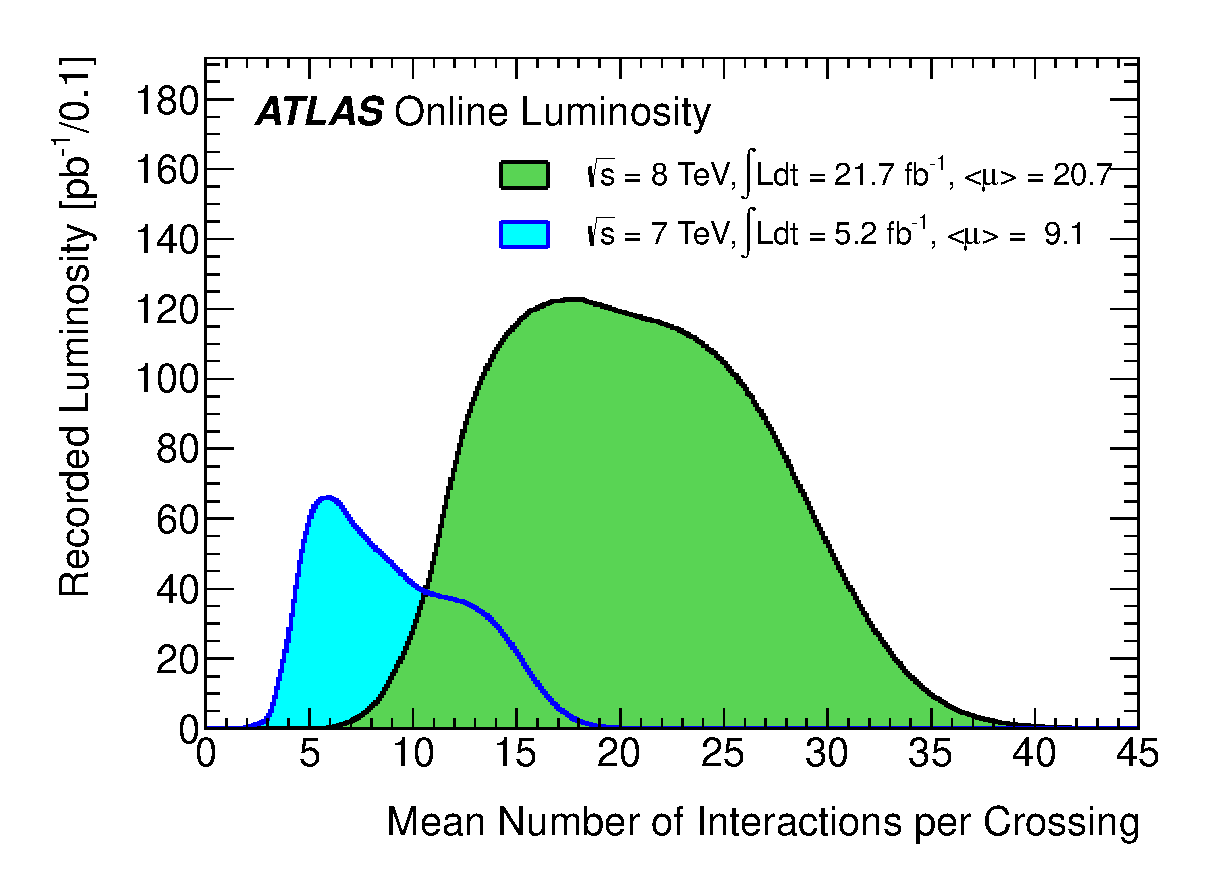
\includegraphics[width=0.49\textwidth]{./figs/mu_2011_2012-dec.eps}
  \label{sfig:meanmu}
}
\subfloat[Integrated luminosity]{
  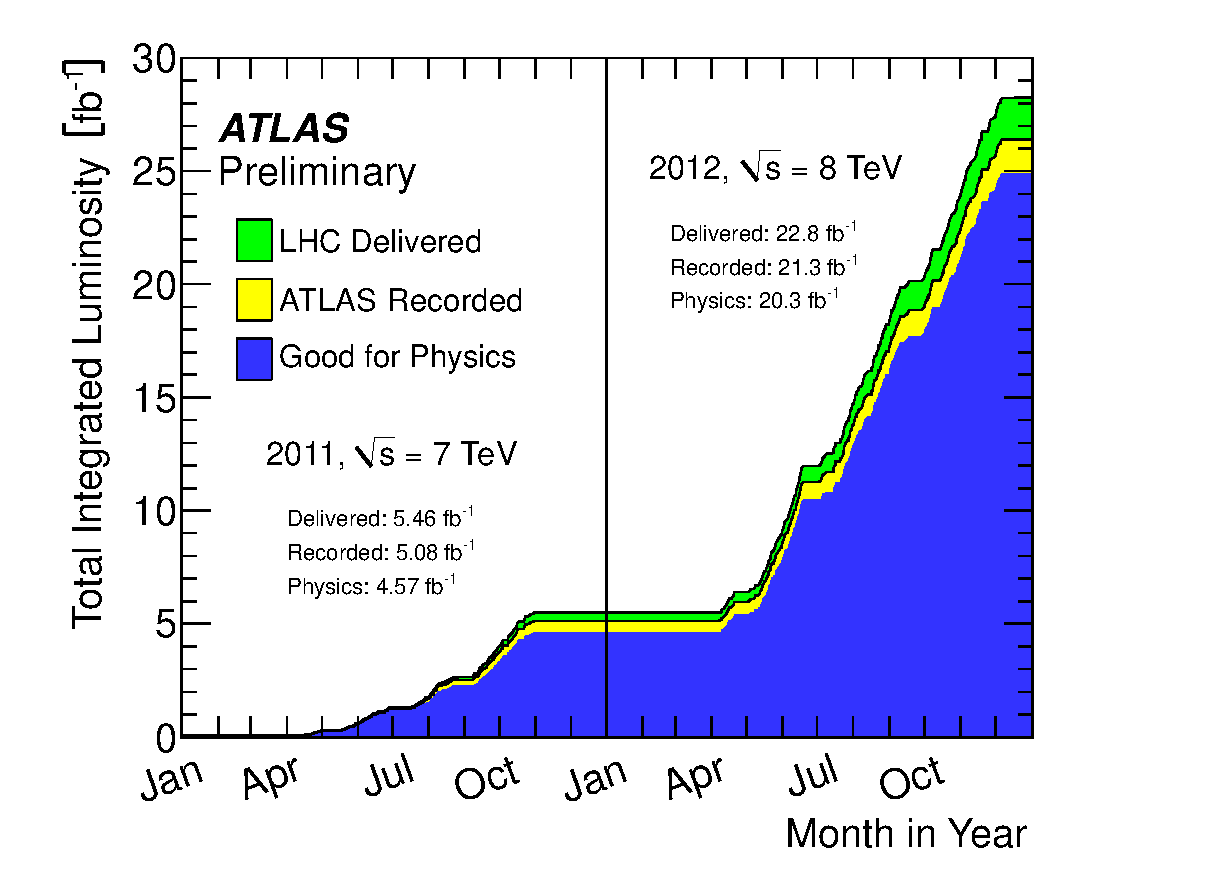
\includegraphics[width=0.49\textwidth]{./figs/intlumivstime2011-2012DQ.eps}
  \label{sfig:cumulumi}
}
\caption[\gls{ATLAS} integrated luminosity and pile-up conditions]{
%
The mean number of interactions per bunch crossing \meanmu~\subref{sfig:meanmu} and the integrated luminosity versus time seen by \gls{ATLAS}~\subref{sfig:cumulumi} for the years 2011 and 2012 with \cmes\ of $\sqrts=7$ and $8$~\TeV~\cite{Aad:2013ucp,ATLASLumiPlots}.
%
\label{fig:cumulumi}}
\end{figure*}
%%%%%%%%%%%%%%%%%%%%%%%%%%%%%%%%%%%%%%%%%%%%%%%%%%%%%%%%%%%%%%%%%%%%%%%%%%%%%
%
The \gls{LHC} has run successfully from 2010 to 2012, a period denoted by \RunOne, with ever increasing performance up to a peak luminosity of $\lumi=7.7\times 10^{33}~\mathrm{cm}^{-2} \mathrm{s}^{-1}$ and a center of mass energy of $\sqrts=8$~TeV. The integrated luminosity versus time delivered by the \gls{LHC}, recorded by \gls{ATLAS} and usable for physics analyses is shown in \fig~\subref*{sfig:cumulumi}. The \gls{LHC} \gls{LS1}, starting in spring 2013, was devoted to upgrading the machine to provide design luminosity and energy. In spring 2015, the first \pp\ collisions of \RunTwo\ at $\sqrts=13$~\TeV\ were recorded and data-taking at the \gls{LHC} experiments started shortly thereafter. Currently, about $\intlumi=4$~\invfb\ of data have already been recorded and are being analysed.
%
The current status of the accelerator and the recorded luminosities of the experiments can be monitored online~\cite{LHCcurr}.
%
The final step to $\sqrts=14$~\TeV\ is planned for early 2016, after the winter shutdown. 
% https://twiki.cern.ch/twiki/bin/view/AtlasPublic/LuminosityPublicResults
% Luminositygroup for citation




\section{The ATLAS detector}
%
The \gls{ATLAS} detector has been designed to optimally study the collisions provided by the \gls{LHC} and search for signatures of new physics. 
%environment
Radiation hard detector components, high resolution in space and time, fast readout electronics and efficient data processing are required to cope with the large event rate provided by the \gls{LHC}. 
%physics goal
The physics goal was most prominently the search for new physics and the \Hboson\ with its experimentally most promising decay channels $H\rightarrow \gamma\gamma$, $H \rightarrow ZZ \rightarrow \ell\ell\ell\ell$, which were the eventual discovery channels, and $H \rightarrow bb$, relevant for a low mass \Hboson. Consequently, the design goals included good photon resolution, $\tau$ lepton identification, highly effective track measurement for electrons and muons and precise \btag. \gls{SUSY} signatures generally involve a large momentum fraction carried by undetectable particles, resulting in large \met. This requires high detector acceptance, leading to the need for maximum spatial coverage around the interaction region and a minimum of uninstrumented material like magnets or support structures inside the detector. 
%
% Besides that, the production of high mass resonances usually takes place at about equally large longitudinal momentum fractions, since collisions involving very high $x$ values are rare, as shown in \fig~\ref{sfig:cteq6mpdf}. The result is a more central emission of the collision products, requiring optimal instrumentation in low pseudorapidity regions.
%
These requirements together with the limitations from available technology determine the key features of the \gls{ATLAS} detector. In the following, the \gls{ATLAS} detector and its main subcomponents in the state of \RunOne\ are described.


%
The cylindrical shape of \gls{ATLAS} with a length of 44~m, a diameter of 25~m and a weight of 7000~t, centred around the interaction point, is displayed in \fig~\ref{fig:ATLASlayout}. The beam axis represents the main axis and the detector components enclose each other in layers of end caps or disks at the fronts and barrels in the center. 
%
\gls{ATLAS} uses a right-handed coordinate system with its origin at the nominal interaction point in the center of the detector and the $z$-axis along the beam pipe. The $x$-axis points from the interaction point to the center of the \gls{LHC} ring, and the $y$-axis points upwards.  Cylindrical coordinates $(r,\phi)$ are used in the transverse plane, with $\phi$ being the azimuthal angle around the beam pipe.  The pseudorapidity is defined in terms of the polar angle $\theta$ as $\eta = -\ln \tan(\theta/2)$.  Angular distances are defined as $\dR \equiv \sqrt{(\Delta\eta)^{2} + (\Delta\phi)^{2}}$.
%
The \gls{ATLAS} detector consists of four main components. As seen from the center of the detector, those are the \gls{ID}~\cite{idtdr1,idtdr2}, the \gls{ECAL}~\cite{calo,LAr}, the \gls{HCAL}~\cite{calo,Tile} and the \gls{MS}~\cite{muon1,muon2}. These are introduced in the following.
%
%
%%%%%%%%%%%%%%%%%%%%%%%%%%%%%%%%%%%%%%%%%%%%%%%%%%%%%%%%%%%%%%%%%%%%%%%%%%%%%%%
\begin{figure*}[tbp!]
\centering
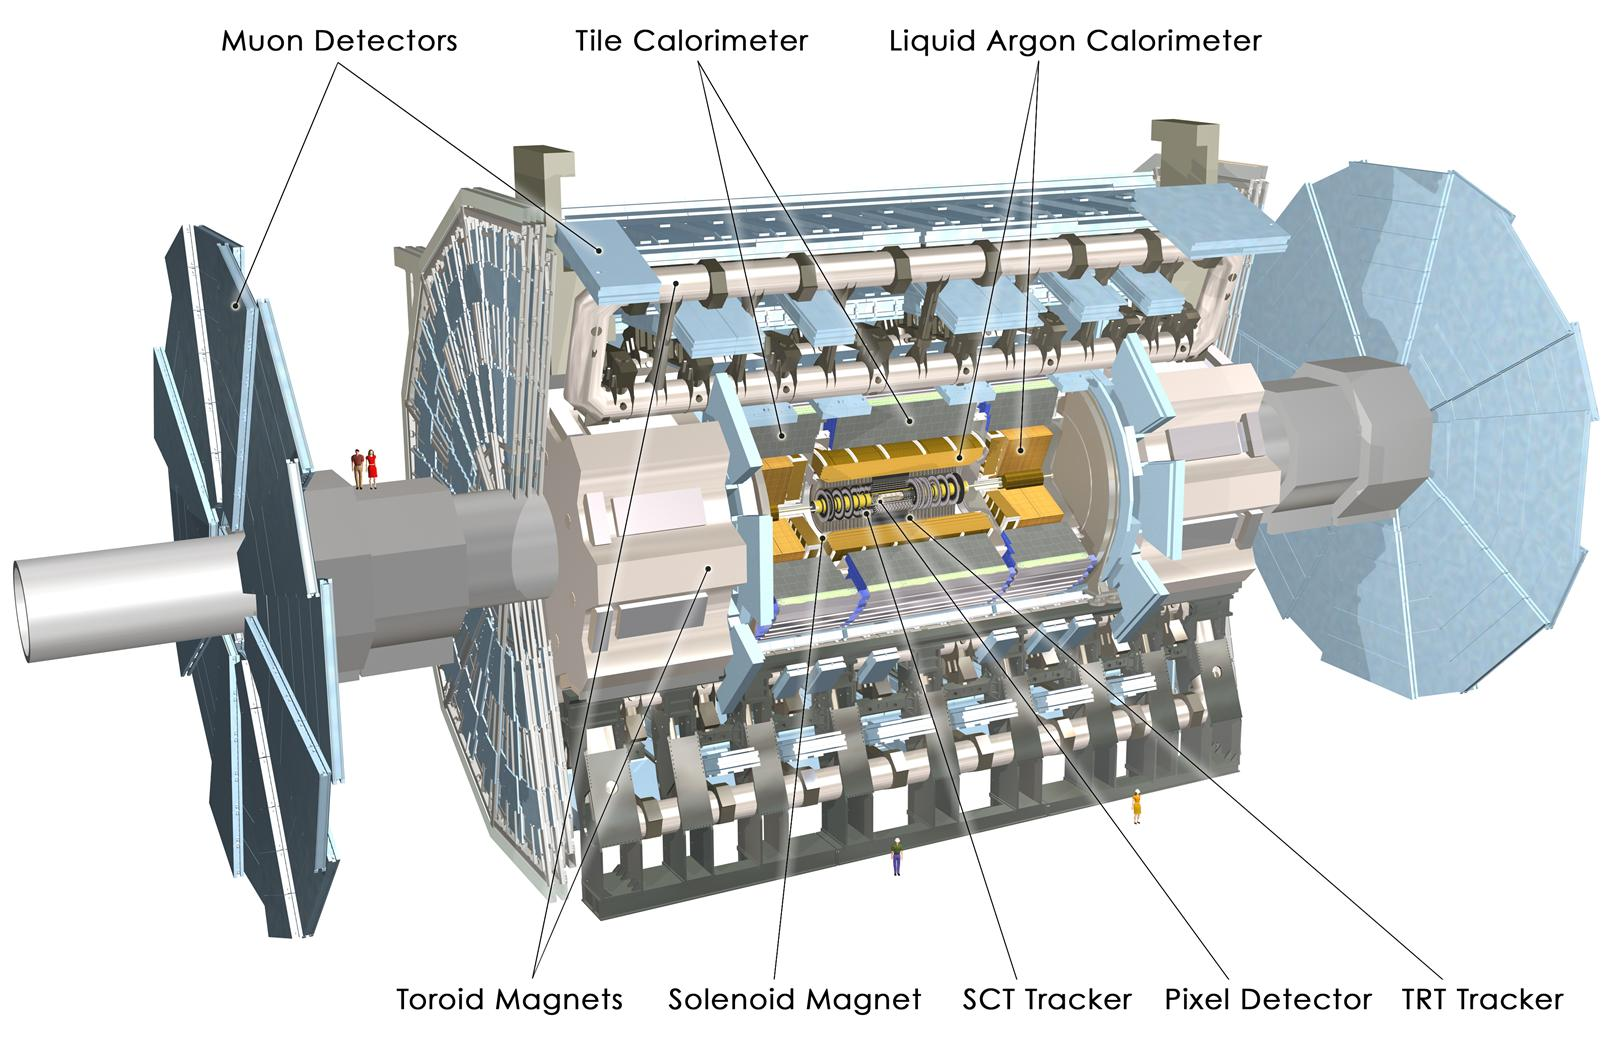
\includegraphics[width=0.8\textwidth]{./figs/ATLAS_full_detector.jpg}
\hfill
\caption[Layout of the \gls{ATLAS} detector]{
%
The layout of the \gls{ATLAS} detector with its main subsystems, enclosing each other around the interaction region in the center~\cite{ATLASpublic}.
%
}
\label{fig:ATLASlayout}
\end{figure*}
%%%%%%%%%%%%%%%%%%%%%%%%%%%%%%%%%%%%%%%%%%%%%%%%%%%%%%%%%%%%%%%%%%%%%%%%%%%%%%%


% best ATLAS reference of all times (no plots, but numbers! Run1 vs Run2):
% https://twiki.cern.ch/twiki/bin/view/AtlasPublic/ApprovedPlotsATLASDetector

\subsection{The inner detector}
%
The innermost $12$~cm in radius are covered by the pixel detector~\cite{pixeltdr}, equipped with three layers of silicon pixel modules and $8.0\times10^7$ readout channels. Radiation damage and multiple scattering is minimised by using very thin pixel layers. The upgrade activities during \gls{LS1} including the installation of a fourth pixel layer with $1.2\times10^7$ readout channels are discussed in more detail in \chap~\ref{chap:trackingupgrades}. 
%
At larger radii, particle tracks can be resolved with less fine and thus less expensive structures. Consequently, four layers of silicon strip detectors are employed in the \gls{SCT}~\cite{sctpaper}, reaching up to $r=52$~cm with about $6.3\times10^6$ readout channels. 
%readout channel info from \cite{Aad:2013ucp}
In the outer region the \gls{TRT}~\cite{trt} is installed. It consists of several hundred thousand drift tubes filled with a Xenon gas mixture, referred to as straws, and operates with $3.5\times10^5$ readout channels. 
%, which can keep up to the delivered luminosity, due to their small diameter of $4$~mm and the distance to the interaction point. 
Radiator foils in between the tubes give rise to Lorentz $\gamma$ dependent transition radiation on particle impact, which is used for the discrimination of electrons and charged pions. 
%
Together with the 2~T magnetic field of the superconducting central solenoid magnet~\cite{Magnet1}, these three sub-detectors provide a fast and precise measurement of charged particle momenta.
%






\subsection{The calorimeter system}
The aim of the calorimeter systems is a necessarily destructive energy measurement of charged and neutral particles, photons and jets via total absorption. 
%
%showers
Particle impact on an absorber generates a shower by the electromagnetic and/or strong interaction. Electromagnetic showers, which are relatively compact and regularly shaped, originate from electrons, photons or electromagnetically decaying pions and scale with the material specific radiation length $X_0$. Hadronic showers, which appear in large irregular shapes, originate from hadrons and are a mixture of hadronically and electromagnetically interacting particles. Consequently, both the nuclear interaction length $\lambda$ and $X_0$ determine the shower evolution. 
%
%non-compensation
Non-ionizing energy losses like nuclear interactions lead to a difference in detector response between electromagnetic and hadronic showers.
%, referred to as non-compensation. 
Together with energy losses in non-instrumented parts like the absorption layers or the magnet coils and other effects, this is compensated for by calibration.
%
%sampling calo
\gls{ATLAS} employs a sampling calorimeter, using different materials for shower production in the absorber and energy measurement in the active layer.
%
%segmentation
For spatial resolution, calorimeters are segmented in cells that can be read out individually to form towers in the direction of the shower evolution. 

These different interaction properties require two different systems, an inner \gls{ECAL} and an outer \gls{HCAL}. 
%
They are installed outside the central solenoid magnet, removing space constraints at the cost of additional particle absorption in the magnet coils. 
%
The \gls{ECAL}~\cite{calo,LAr} is designed to fully absorb any electromagnetic shower and prevent the generation of secondary hadronic showers. Its accordion shaped layers consist of lead plates as absorber and \gls{LAr} in between as active material. 
%
The \gls{HCAL}~\cite{calo,Tile} determines the energies of hadrons. The barrel region uses copper or tungsten as absorber material and tiles of scintillating plastic as sensors. The forward region is covered by the \gls{HEC}, which is a \gls{LAr} calorimeter with copper plates as absorbers.
%









\subsection{The muon system}
Complementing the muon track measurement in the \gls{ID}, an additional large tracker system is employed to measure the muon momentum and charge~\cite{muon1,muon2}. Especially for large momenta, the resolution of a track measurement from the curvature is determined by the superconducting air core toroid magnet system~\cite{Magnet1}. The magnet system provides a bending power of up to 6~Tm in a toroidal volume extending radially from 9 to 20~m and longitudinally across a length of 25~m, while at the same time minimising multiple scattering. 
%
The bent muon tracks are measured with three layers of \gls{MDT}, consisting of high pressure proportional drift tubes. The  individual drift tubes have a diameter of 3~cm and their sense wires are aligned with a precision similar to the required sagitta precision of 10 to 30~\mum, using a laser position monitoring system for offline correction.
% Due to the high occupancy in the forward region, Cathode Strip Chambers (\gls{CSC}) are employed here which have a smaller segmentation.
Additional \gls{RPC} and \gls{TGC} systems are used for fast muon trigger decisions. They are further used to identify the bunch crossing of interest and provide additional tracking information.
% MDT: https://cds.cern.ch/record/319197/files/muon-96-129.pdf
%useful site: http://www.atlas.ch/t_barrel.html










\subsection{Trigger system and computing}
The physically interesting high mass resonances are rare compared to the total number of collisions. As shown in \fig~\subref*{sfig:xsecs}, the total inelastic \pp\ cross section at the \gls{LHC} is about $70$~mb and the first relevant hard scattering, the \Wboson\ scattering, occurs with a cross section of about $100$~\nb~\cite{Dittmaier:2012nh}. To overcome this abundance of \gls{QCD} background and to match the maximum event recording frequency of $400$~Hz, the trigger decisions in the \gls{DAQ} system provide an efficient event preselection. Triggers are sets of decision criteria, leading to detector buffer read out and subsequent data storage. \gls{ATLAS} employs a three step trigger system~\cite{ATLASCSC}. 
%
The level 1 trigger uses hardware based information on coincidences of single subsystem signals from the \glspl{RPC}, the \glspl{TGC} or the calorimeters for a decision within $2.5$~$\mu$s, reducing the event rate from the bunch crossing rate of about $40$~MHz to about $75$~kHz. Due to this, all detector components are equipped with buffers to store events locally and to pass them on to the  \gls{DAQ} system if a trigger signal arrives. 
%
These events are then subject to the software based level 2 trigger and the \gls{EF}, collectively referred to as \gls{HLT}. The required event processing is performed on computing farms. 
%
The level 2 trigger reduces the event rate from about $75$ to about $2$~kHz, based on an analysis of event topologies in \gls{ROI} defined by the level 1 trigger, requiring only some percent of the full event information.
%
The last stage is the \gls{EF} which applies an in-depth analysis of the event using information on calibration, alignment and magnetic field topology. This leads to a final event storage rate of about $300$ and $400$~Hz for data recording in the years 2011 and 2012, respectively, corresponding to a full event data volume of a few hundred MB/s.
%http://arxiv.org/pdf/1406.5375v2.pdf


A distributed computing grid, the \gls{WLCG}, has been set up to grant easy access, reliable data storage and high performance data processing to the more than 10,000 users. This comes with a number of challenges, especially requirements of high bandwidth, software compatibility and the balance of resources. The \gls{WLCG} spans more than 170 computing centers in 42 countries with a hierarchy dependent on the capabilities of the respective site, managing more than 2 million computing jobs every day and about 30~PB of data per year~\cite{WLCGwebsite}.
% http://wlcg.web.cern.ch/

























